% 来源：固定1991上海PDF第2页（印刷5-34），第24题。
% 忠实投影复现：原图仅有AB、AC、BC、BD、CD五条实线。
% 不补AD、H、R或解析辅助线；投影坐标不增加度量条件。
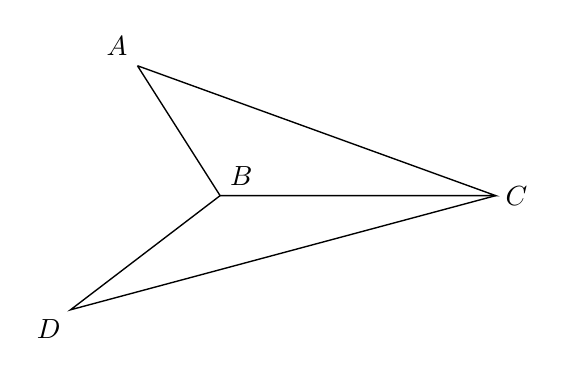
\begin{tikzpicture}[line width=0.5pt,scale=1.0]
  \coordinate (A) at (0.2,2.3);
  \coordinate (B) at (1.25,0.65);
  \coordinate (C) at (4.75,0.65);
  \coordinate (D) at (-0.65,-0.8);
  \draw (A)--(B)--(C)--(A);
  \draw (B)--(D)--(C);
  \node[above left] at (A) {$A$};
  \node[above right] at (B) {$B$};
  \node[right] at (C) {$C$};
  \node[below left] at (D) {$D$};
\end{tikzpicture}
